\documentclass[conference]{IEEEtran}
\usepackage[T1]{fontenc}
\IEEEoverridecommandlockouts
% The preceding line is only needed to identify funding in the first footnote. If that is unneeded, please comment it out.
\usepackage{cite}
\usepackage{amsmath,amssymb,amsfonts}

\usepackage[linesnumbered,ruled,vlined]{algorithm2e}
\DontPrintSemicolon
\usepackage[hidelinks]{hyperref}
\usepackage[noabbrev,capitalize]{cleveref}
\usepackage{array, booktabs, makecell}
\usepackage{graphicx}
\usepackage{textcomp}
\usepackage{xcolor}
\usepackage{caption}
\usepackage{subcaption}

\usepackage{tikz}
\usetikzlibrary{trees}

\newcommand\norm[1]{\left\lVert#1\right\rVert}
\def\BibTeX{{\rm B\kern-.05em{\sc i\kern-.025em b}\kern-.08em
    T\kern-.1667em\lower.7ex\hbox{E}\kern-.125emX}}

\graphicspath{../}
\hypersetup{
    colorlinks=true,
    linkcolor=black,
    filecolor=black,      
    citecolor=black,
    urlcolor=blue,
    pdfpagemode=FullScreen,
    }

\begin{document}

\title{Parallel Huffman Coding}

\author{\IEEEauthorblockN{Francesco Bozzo}
    \IEEEauthorblockA{\textit{DISI, University of Trento} \\
        Trento, Italy\\
        francesco.bozzo@studenti.unitn.it\\
        229312}
    \and
    \IEEEauthorblockN{Michele Yin}
    \IEEEauthorblockA{\textit{DISI, University of Trento} \\
        Trento, Italy\\
        michele.yin@studenti.unitn.it\\
        229359}
}

\maketitle

% add page number
\thispagestyle{plain}
\pagestyle{plain}

\begin{abstract}
    This report aims to explain the design of a parallel encoding and decoding Huffman algorithm. The application is developed with the C99 programming language, using MPI for multiprocessing and OpenMP for multithreading to scale horizontally with increasing hardware resources. Our tool is both able to exploit multiprocessing to process concurrently multiple files, and to split the Huffman coding of the same file among multiple threads.

    Comparing this tool with other online implementations, we can state that\dots
\end{abstract}

\begin{IEEEkeywords}
    Huffman, MPI, OpenMP, High Performance Computing
\end{IEEEkeywords}

\section{Introduction}
Even if the Huffman algorithm is not directly used nowadays, its prefix mechanism is still part of Deflate (PKZIP's algorithm), JPEG, and MP3 compression algorithms


\section{The Huffman algorithm}
The Huffman algorithm has the objective of finding a more convenient bit representation to store information through lossless compression. Instead of considering groups of eight bits as the way to encode data, the Huffman algorithm uses variable-length sequences of bits with prefixes defined as \emph{alphabet}.

\subsection{Priority Queue}
The Huffman algorithm uses a minimum priority queue to build its alphabet efficiently. This specific data structure ensures logarithmic insertion and deletion time with respect to its size.
We implemented the minimum priority queue by using a minimum heap. Practically speaking, to implement the min-heap tree, we used a standard C array ensuring that the min-heap property still holds at every insertion and deletion:
\begin{equation}
    A[i] \le A[l(i)], A[i] \le A[r(i)]
\end{equation}
where \(A[i]\), \(A[l(i)]\), \(and A[r(i)]\) are respectively a node, its left child, and its right child in a min-heap tree.

To implement the priority queue also a parallel approach has been considered \cite{BRODAL19984}, but since it contains only 256 elements, we did not consider it too important in terms of performance.

\subsection{Encoding}
The Huffman encoding procedure makes use of a minimum priority queue to build its alphabet efficiently. The idea is to build a tree similar to \cref{fig:tree} that defines all the variable-length prefix sequences of bits: these sequences are represented by the path from the tree root to a leaf. Using a greedy approach, the Huffman encoding ensures that the less frequent a byte is in a file, the more probable is to have a longer Huffman representation, which means that his path from the root to its specific leaf is longer.

Once having computed the frequencies for each one of the 256 different bytes in a file, the Huffman algorithm populates a min priority queue with Huffman tree nodes storing the byte value and its frequency. Successively, it removes the least two frequent bytes from the queue, creates a new node with children the two extracted nodes, assigns to it a dummy character and the sum of the frequencies of its two children, and inserts it into the min priority queue. After \(n-1\) iterations, the last node is the root of the Huffman tree \cite{bertossi2010algoritmi}. \Cref{alg:buildtree} explains in the detail this procedure.
\begin{algorithm}
    \caption{Build the Huffman tree}\label{alg:buildtree}

    \SetKwData{Q}{Q}\SetKwData{z1}{z1}\SetKwData{z2}{z2}\SetKwData{z}{z}
    \SetKwFunction{insert}{insert}\SetKwFunction{deleteMin}{deleteMin}
    \SetKwInOut{Input}{input}\SetKwInOut{Output}{output}
    \SetKwFor{}{}{}{}

    // Populate the min priority queue with characters and their frequencies\;
    \For{\(i=1\) \KwTo \(n-1\)}{
        Q.insert(f[i], Tree(f[i], c[i]))\;
    }
    // Repeat until the queue has only a single element left\;
    \For{\(i=1\) \KwTo \(n-1\)}{
        // Get the two least frequent nodes\;
        z1 = Q.deleteMin()\;
        z2 = Q.deleteMin()\;

        // Create an inner tree node and insert it into the queue\;
        z = Tree(z1.f + z2.f, null)\;
        z.left = z1\;
        z.right = z2\;
        Q.insert(z.f, z)\;
    }

    // The last element in the queue is the root of the Huffman tree\;
    \Return{Q.deleteMin()}\;
\end{algorithm}

Once built the Huffman tree, it is possible to generate the Huffman alphabet visiting the tree using a DFS algorithm, assigning 0 to each left-child traverse and 1 for the right one as presented in \cref{alg:encode}. Finally, it is possible to compress the file by creating a stream of bits corresponding to its content using the Huffman alphabet.

\begin{algorithm}
    \caption{Encode using Huffman tree}\label{alg:encode}
    \While{not eof()}{
        bit = read()\;
        \eIf{bit == 0}{
            encode(node.left)\;
        }{
            encode(node.right)\;
        }
        \If{node is leaf}{
            \Return{node.value}\;
        }
    }
\end{algorithm}

\begin{center}
    \begin{figure}
        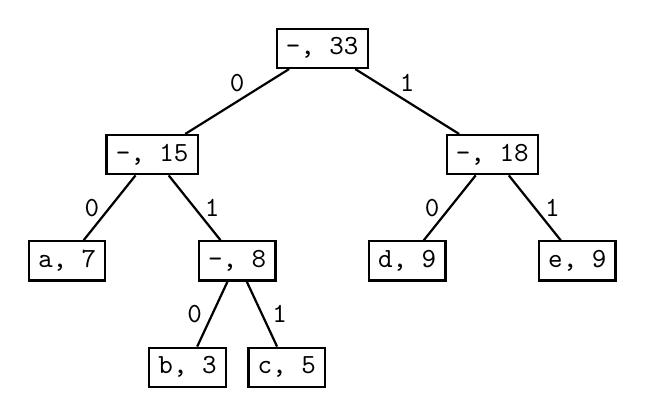
\begin{tikzpicture}
            [
                level distance=1.5cm,
                level 1/.style={sibling distance=4.8cm},
                level 2/.style={sibling distance=2.4cm},
                level 3/.style={sibling distance=1.4cm},
                thick,
                font=\ttfamily\bfseries, scale=0.9
            ]
            \tikzset{
                treenode/.style = {rectangle, draw=black, align=center,minimum width=0.75cm},
                edgestyleL/.style = {midway,left,draw=none},
                edgestyleR/.style = {midway,right,draw=none}
            }
            \node [treenode] (T) {-, 33}
            child { node[treenode] (L) {-, 15}
                    child { node[treenode] (LL) {a, 7} edge from parent node[edgestyleL] {0} }
                    child { node[treenode] (LR) {-, 8}
                            child { node[treenode] (LRL) {b, 3} edge from parent node[edgestyleL] {0} }
                            child { node[treenode] (LRR) {c, 5} edge from parent node[edgestyleR] {1} }
                            edge from parent node[edgestyleR] {1}
                        }
                    edge from parent node[edgestyleL,above] {0}
                }
            child { node[treenode] (R) {-, 18}
                    child { node[treenode] {d, 9} edge from parent node[edgestyleL] {0}}
                    child { node[treenode] {e, 9} edge from parent node[edgestyleR] {1}}
                    edge from parent node[edgestyleR,above] {1}
                }
            ;
        \end{tikzpicture}
        \caption{An example of Huffman tree.}
        \label{fig:tree}
    \end{figure}

\end{center}

\subsection{Decoding}
Once having the encoded file and the Huffman tree, it is straightforward to decompress the file to its original shape. The prefix alphabet ensures to have that it is possible to visit the tree using a DFS approach and get a unique decoded version of the file using an approach similar to \cref{alg:encode}.

\section{Serial Huffman implementation}
To be able to implement the Huffman encoding and decoding algorithm, several things have been taken into account.
\begin{itemize}
    \item The byte frequencies computed during the encoding process are saved in the compressed file. In this way, the decoding procedure can easily rebuild the Huffman tree.
    \item Both the encoding and decoding procedures make use of buffers to improve I/O performance: the streams of bytes are first written inside the buffer and then saved on the disk.
    \item The encoding procedure works with chunks of \(4096\) bytes. This ensures that the tool can handle even large files when dealing with bit buffers. The decoding procedure deals with chunks of maximum size of \(4096*32\) bytes, since the maximum length of a Huffman tree traverse from root to leaf is of 256 bits, which is 32 times a byte. As explained later, dealing with chunks makes handy the parallel implementation of the encoding and decoding algorithms.
    \item In the encoded file, the chunk offsets are saved at the end of the file: this ensures that the compressed stream of prefixed sequences of bits is still meaningful.
\end{itemize}

\section{Parallel Huffman Implementation}
To parallelize our algorithm over threads and processes, we decided to follow this simple yet effective structure
\begin{itemize}
    \item multiple processes will process groups of file and folders separately.
    \item multiple threads of the same process will compute different chunk of the same file in parallel.
\end{itemize}

There are a many reasons to our choice. Mainly they are:

\begin{itemize}
	\item In most operating systems a file is a resource that the OS gives to a single process. We wanted to follow a similar design philosophy.
	\item Most operating system can allow multiple processes to open the same file in reading mode, but few allow to multiple processes to open the same file in writing mode. This is because that leads to potentially concurrency and data integrity issues. By having only a single process open a single file, we avoid all these issues.
	\item Because threads of the same process share the address space, we can avoid the expensive data transfer across processes. When data is read or written to file, there is no need to transfer data between threads.
\end{itemize}

We start by explaining the basic multithreading operations on a single file and then we'll cover multiprocessing with multiple files.

\subsection{Multithreading}

The parallel algorithm for a single file follows the same exact procedure as a serial version, but with few key differences to allow multithreading.

A single file is divided in chunks of a fixed size. When that is done, the single process forks and creates the number of threads we intented.

One of them reads a number of chunks equal to the team size. When it's done reading the chunks, all threads can work on the processing in parallel. 

Every chunk is processed by a single thread, that reads and writes on the shared memory space of its process. Although all the chunks are in shared memory, each thread is assigned a single chunk and it processes only data in own chunk to avoid any concurrency related problems.

When all threads are done  computing either the encoding or decoding of their chunks, a single thread writes the processed chunks to the output file.
Again, because all threads share a memory space there is no need to perform data transfer.


The overall procedure is the same in both encoding and decoding, with very small differences. 

We also parallelized the counting of occurences of a byte in the input file, that is required in order to create the huffman tree, with a similar architecture.  Key difference is that there is no output file to write, but only occurences to count.

In figure \ref{fig:threading}a schema of the architecture. 

\begin{figure}
	\centering
	\includegraphics[width=0.8\linewidth]{../imgs/threading}
	\caption{Simple schema of the threading paradigm.}
	\label{fig:threading}
\end{figure}


\subsection{Multiprocessing}

For multiple files we wanted to exploit multiprocessing.

To do this we devised a simple algorithm to distribuite files across multiple processes, so that each process can work on its own list of files, indipendently to others. This way we can minimize communcation and therefore latency and other slowdowns.


First of all the process with rank 0 crawls all the files present in the input directory recursively. Then it opens all the files and reads their size. 

Once all files and their respective sizes are known, the process creates a min priority queue where each item represents a process and its priority is the  size of files that have been assigned to it.

Process 0 can iteratively insert files in the priority queue and updates the priority of each process with the cumulative file size. This way we can ensure an almost equal work division among different processes. 

When all this is done, process 0 sends the list of files to each process and then each starts to work indipendetly on its own list of files.



\subsection{Implementation details and other notes}

\begin{itemize}

\item We found that a chunk size of 4096 Byte had the best I/O times. This is probably due to the fact that 4096 B is the size of a page in most Linux based operating systems. The last chunk of a file may be smaller. Reading any other size at the time had resulted in significanlty worse I/O times ( both increasing and decreasing the chunk size ).

\item In general, all threads will finish processing their chunk at around the same time, but in some cases, there are threads that can take longer. This is due to the very unlucky case where a whole chunk contains exclusively very infrequent characters or bytes of data. Because the bytes are very infrequent each is encoded in extremely long sequences, up to 256 bits, resulting in a bigger encoded chunk than compared to the original data. With our alphabet at 1 Byte, the worst case results in a chunk that is 32 times bigger than original.

\item We tried to parallelize the I/O, by having each thread read its own chunk. We found that the standard file descriptor provided by C have a lock to guarantee thread safety.  This lock slows down the reads significantly. We also tried using multiple file descriptors to circumvent this limitation, however we found no improvement over a sequential read done by one thread for all the threads in it's team. This is likely because the O.S. schedules I/O requests and serves them one at the time, resulting in a impossiblity of having truly parallel I/O.

\item We also tested an architecture where we had two dedicated threads to I/O, one for reading and one for writing chunks. The idea is that whenever a chunk is processed, the I/O threads would immediately write the processed chunk to the output file and similarly a new chunk would be read from the input file. Theoretically this would allow to parallelize I/O and computation operations and we avoided concurrency problems by synchronizing the I/O with locks. However we found that this approach was a waste  of resources, as the I/O on the cluster is extremely fast ($\sim$ 5 GiB +/s) and it resulted in the I/O threads being idle most of the time, waiting for a chunk to be processed. Although we discarded this architecture, it may be useful in systems or problems where I/O operations take a significant amount of time or at least comparable to processing operations. 
\item Another noticeable detail we noticed on the implementation with two dedicated threads for I/O, is that if there are not enough cores on the CPU or if the operating system decides to allocate all the threads on a single processor, the encoding and decoding times are greatly affected by the scheduler. This is because it might be that the O.S. gives priority to threads that are waiting ( for example the writer cannot write any block until the first has finished, even if all others have finished)

\end{itemize}

\section{Performance and benchmarking}
Here we discuss the perfomance evaluation of our algorithm.
We start from a evaluation of some other implementations of Huffman algorithm and then focus on the analysis of our own implementation. 

We include in this section some graphs and statistics but all detailed results are included in the appendix at the end this report.
\subsection{setup}
All data is resulting average of 3 runs to minimize the effect random variance in between runs.
We tested everything on HPC2 cluster of University of Trento.
We also used a single node, using the \verb|--map-by | command to map the correct number of cores to each MPI process.
Each time we submitted as a job to the cluster individually, waiting for the previuos to finish. This is to prevent hiccups due to multiple instances of the program trying to access the same data, which we noticed greatly affect I/O times.

The correctness of our algorithm was easily verified by encoding and then decoding a file, then comparing the decoded result to the original with the \verb|diff| command.
\subsection{datasets}
The dataset was pragmatically generated using a C program , creating text files with characters that follow the frequency of letters in English language. Although for this benchmark are only using the 26 letters of the English alphabet, our algorithm reads bytes of data and can therefore work con any type of file.

In particular we chose to analyze these file sizes 1 MiB, 5 MiB, 10 MiB , 50 MiB, 100 MiB, 500 MiB, 1 GiB, 5 GiB, 10 GiB. This should be enough range to understand different algorithms scale with increasing file sizes.

Secondly, because our algorithm also works with many files at once, we used Linux kernel as benchmark for that scenario. As the time of writing, it is about 1.3 GiB of total size, with about  $\sim$ 84.000 files, which on average are each 16MiB in size.

Considering the dataset sizes and testing we have done, we estimate to have read or wrote about $\sim$ 6 TiB of data for our whole benchmark analysis.
\subsection{Other works}

\subsection{Multithreading evaluation}
In this section we evaluate our algorithm on single files, using multithreading and testing our parallelization perfomances with increasing number of threads available.

We can say that with small files, less than a few MiBs, the algorithm is actually slower with more threads. 
This is likely because the data is not large enough to offset the cost of creating multiple threads. Considering the cost parallel processing, we highly suggest not doing parallelization for small files.

However when the data is large enough our multithreaded approach scales up.

With the largest file (10 GiB) our algorithm has an efficiency of 93\% when tested with 4 threads. This number steadily decreases with the number of threads and we hit 32\% with 24 threads.

It has to be noted that we are heavily limited by the I/O. As we are unable to parallelize the I/O, we are heavily limited by that. Especially writing to disk taskes a considerable amount of time.

As a proof of this, if we consider only the processing section of our algorithm, and ignore the time required by the \verb|fflush()| operation before a \verb|fclose()|, we see significantly better times. Although we start from similar efficiency at low threading, we achieve a 54\% efficiency with 24 threads.

\begin{figure}
	\centering
	\includegraphics[width=0.8\linewidth]{"../imgs/Flush vs non Flush"}
	\caption{Encoding times with and without the flush()}
	\label{fig:flush-vs-non-flush}
\end{figure}

If we consider only CPU time, which doesn't count the time spent waiting in I/O, we get incredibile results.
 
We also noticed worse times in decoding than encoding. This is probably due to the fact that we are reading fixed chunks of 4096 bytes in encoding, but when we decode, we read the same chunks which is now of a different size than 4096 bytes. 

\begin{figure}
	\centering
	\includegraphics[width=0.8\linewidth]{"../imgs/Encoding vs Decoding"}
	\caption{Encoding vs Decoding times}
	\label{fig:encoding-vs-decoding}
\end{figure}

As cited in the previous section, we also tested a version with lock based synchronization instead of barrier. Although theoretically we should get better results, in practice we almost equal results across the board, with only the largest file having some significant difference. This difference is greater in decoding than in encoding.
\begin{figure}
	\centering
	\includegraphics[width=0.8\linewidth]{"../imgs/Barrier vs Locks encoding"}
	\caption{Barrier vs Lock based synchronization perfomance}
	\label{fig:barrier-vs-locks-encoding}
\end{figure}

\begin{figure}
	\centering
	\includegraphics[width=0.8\linewidth]{"../imgs/Encoding Barrier times"}
	\caption{Encoding times}
	\label{fig:encoding-barrier-times}
\end{figure}

\subsection{Multiprocesssing}
We tested on Linux kernel as benchmark the parallelization perfomances of our algorithm. Theoretically our algoritm should scale very well with increasing number of processes and files, because once the main process sends the list of files to encode to each process there is no further communication between different processes. However we find that real world results are different. 
While we don't expect much perfomances by increasing the number of threads, because the files are on average very small, we should get better results by using many processes.
With increasing number of processes, our algorithm does not scale at all. We believe the main limitation of our algorithm is the I/O of the cluster we tested on. When tested on a local machine \footnote{MacBook A2442} with one thread and 1,2,4 processes, we find that our algorithm does indeed scale with the number of processes. 
\subsection{Memory, storage and other considerations}
Our memory requirements don't scale upwards with the size of the files we need to encode, because at any given time, the most we only store is the size of two buffers, each is a \verb|unsigned char buffer[num_threads][4096]|. These buffers are emptied at each I/O cycle, therefore leading to a high memory efficiency. Only when processing multiple files our memory requirements scale up with the number of files, as each process needs to store information about the files is assigned to process.

We also find that we achieve on average 48\% compression rate of our synthetic data. Instead on Linux kernel, because contains more varied data which consists of mostly code, we achieve a lower 62\% compression rate. Testing on other already compressed data as \verb|.zip| or \verb|AV1| resulted in a compression rate of 100\%.
\input{sections/conclusion}

\bibliography{bibliography.bib}{}
\bibliographystyle{IEEEtran}

\end{document}
